% 非互換なパッケージに自動でパッチを当てる
% https://qiita.com/wtsnjp/items/76557b1598445a1fc9da
\RequirePackage{plautopatch}
% pdfpagesの依存パッケージのエラー回避
% https://okumuralab.org/tex/mod/forum/discuss.php?d=2956
% https://github.com/aminophen/gentombow/issues/9
\plautopatchdisable{eso-pic}
% documentclassでdvipdfmx指定をするので個別パッケージでのドライバ指定は不要
% https://qiita.com/Aruneko/items/13e015bce0112143f277
\documentclass[autodetect-engine, dvi=dvipdfmx, 10pt, a4paper, ja=standard]{bxjsarticle}

% 印刷時の用紙サイズ設定
\usepackage{bxpapersize}% これでOK!

% pdf-version
\usepackage[1.4]{bxpdfver}

% 日本語環境での字体修正
\usepackage{otf}
% フォントエンコーディングの名前をオプションで指定する
\usepackage[T1]{fontenc}
\usepackage{lmodern}% Latin Modern フォントを使う

% graphicx
\usepackage{graphicx}
\usepackage{grffile}% include graphicsの画像ファイル名の制限を撤廃

% \begin{comment} ... \end{comment} で複数行コメントアウト
\usepackage{comment}

% 数学系 インライン数式を \[ \] と書く癖をつける
\usepackage{amsmath,amssymb,amsthm}
\usepackage{amsfonts}
\usepackage{mathtools}
\usepackage{bm} % bold math

% 化学
\usepackage[version=4]{mhchem}

% SI単位系
\usepackage{siunitx}

% 表関連
\usepackage{multirow} % 表のセルの結合
\usepackage{booktabs} % 表の線がすごくなる. Table Generatorを使うときはbooktabsモードにする
\usepackage{caption} % キャプションをいじる
\usepackage{float} % 図表を絶対にそこに置く確固たる意思

% その他便利な子
\usepackage{pdfpages} % pdfを挿入
\usepackage[hyphens]{url} % urlをきれいに表示する
\usepackage{ulem} % 下線を強化
\usepackage[at]{easylist} % @をつかって箇条書き
% \usepackage{minted}
% \usepackage{termsim} % ターミナルを再現...誰得?

% ハイパーリンクを生成
% sectionなどで数式を使う場合は \texorpdfstring{texstring}{pdfstring}をする
\usepackage{hyperref}
\usepackage{pxjahyper}
\usepackage{footnotebackref} % 脚注から本文へ飛べる


% ここからはソースコードを表示する設定
\usepackage{listings, plistings, color}
\renewcommand{\lstlistingname}{Code}
\definecolor{OliveGreen}{rgb}{0.0,0.6,0.0}
\definecolor{Orenge}{rgb}{0.89,0.55,0}
\definecolor{SkyBlue}{rgb}{0.28, 0.28, 0.95}
\lstset{
    language={Ruby}, % 言語の指定
    basicstyle={\ttfamily},
    identifierstyle={\small},
    commentstyle={\smallitshape},
    keywordstyle={\small\bfseries},
    ndkeywordstyle={\small},
    stringstyle={\small\ttfamily},
    frame={tb},
    breaklines=true,
    columns=[l]{fullflexible},
    numbers=left,
    xrightmargin=0zw,
    xleftmargin=3zw,
    numberstyle={\scriptsize},
    stepnumber=1,
    numbersep=1zw,
    lineskip=-0.5ex,
    stepnumber=1,       % 行数の増間
    numbersep=1zw,      % 行数の余白
    xrightmargin=0zw,   % 左の余白
    xleftmargin=2zw,    % 右の余白
    framexleftmargin=18pt,  % フレームからの左の余白
    keepspaces=true,    % スペースを省略せず保持
    lineskip=-0.2ex,    % 枠線の途切れ防止
    tabsize = 4,        % タブ数
    showstringspaces=false,  %文字列中の半角スペースを表示させない
    keywordstyle={\color{SkyBlue}},     %キーワード(int, ifなど)の書体指定
    commentstyle={\color{OliveGreen}},  %注釈の書体
    stringstyle=\color{Orenge}          %文字列
}

% \refだけで「図」や「式」を自動挿入
% https://zenn.dev/arks/articles/3697b25d03f8a8
% subfigureが文書にあると小節を参照する際に使う\subrefがおかしくなるので注意
%% increase link area for cross-references and autoname them, [130514]
\AtBeginDocument{\renewcommand{\ref}[1]{\mbox{\autoref{#1}}}}

\def\equationautorefname~#1\null{式(#1)\null}
\def\figureautorefname~#1\null{図#1\null}
\def\subfigureautorefname#1\null{図#1\null}
\def\tableautorefname~#1{表#1}
\def\lstlistingautorefname~#1{コード#1}

\def\partautorefname#1\null{第#1部\null}
\def\chapterautorefname#1\null{第#1章\null}
\def\sectionautorefname#1\null{#1節}
\def\subsectionautorefname~#1\null{#1節}
\def\subsubsectionautorefname#1\null{#1節}
\def\paragraphautorefname#1\null{#1段落}
\def\subparagraphautorefname#1\null{#1段落}

\def\Itemautorefname#1\null{項目#1\null}
\def\Hfootnoteautorefname#1\null{脚注#1\null}
\def\theoremautorefname#1\null{定理#1\null}
\def\FancyVerbLineautorefname#1\null{#1行\null}
% \def\pageautorefname#1\null{ページ#1\null}
\def\appendixautorefname#1\null{付録#1\null}


\title{MICS実験第一 J8課題レポート}
\author{学籍番号 2210342, 鈴木謙太郎}
\date{\today}
\begin{document}
\maketitle


\section{課題1}
\label{sec:ex-1}

実験資料を参考に,\ref{code:ex-1}のようにremove\_edge関数及びreorient\_edge関数を実装した.


\begin{lstlisting}[language={C}, caption={実装したremove\_edge関数及びreorient\_edge関数のソースコード}, label={code:ex-1}]
void remove_edge(graph *g, int x, int y) {
  if (is_edge(g, x, y)) {
    int i;
    for (i = 0; i < g->degree[x]; i++) {
      // is_edge(g, x, y)が真であるので,g->degree[x][i] == yとなるiは必ず存在
      // よって必ずbreakするしこのfor-loopは安全
      if (g->edges[x][i] == y) {
        break;
      }
    }
    for (; i < g->degree[x] - 1; i++) {
  	  g->edges[x][i] = g->edges[x][i + 1];
    }
    g->degree[x]--;
    g->nedges--;
    return;
  }
  fprintf(stderr, "Warning: (%d, %d) does not exist\n", x, y);
}

void reorient_edge(graph *g, int x, int y) {
  if (is_edge(g, x, y)) {
    remove_edge(g, x, y);
    insert_edge(g, y, x);
  } else {
    fprintf(stderr, "Warning: (%d, %d) does not exist\n", x, y);
  }
  return;
}
\end{lstlisting}

また,配布されたテストプログラムを用いてこれらの関数を含む処理を実行した結果は以下のようになった.

\begin{verbatim}
> ./kadai1main kadai1/input.txt
0: 1 2
1: 3 5
2: 3 4
3: 4
4: 5
5: 7
6: 4 5
7:
degree[0]: 2
degree[1]: 2
degree[2]: 2
degree[3]: 1
degree[4]: 1
degree[5]: 1
degree[6]: 2
degree[7]: 0
nedges = 11
***** insert an edge (input two numbers):
0 3
0: 1 2 3
1: 3 5
2: 3 4
3: 4
4: 5
5: 7
6: 4 5
7:
degree[0]: 3
degree[1]: 2
degree[2]: 2
degree[3]: 1
degree[4]: 1
degree[5]: 1
degree[6]: 2
degree[7]: 0
nedges = 12
***** remove an edge (input two numbers):
0 1
0: 2 3
1: 3 5
2: 3 4
3: 4
4: 5
5: 7
6: 4 5
7:
degree[0]: 2
degree[1]: 2
degree[2]: 2
degree[3]: 1
degree[4]: 1
degree[5]: 1
degree[6]: 2
degree[7]: 0
nedges = 11
***** reorient an edge (input two numbers):
0 2
0: 3
1: 3 5
2: 3 4 0
3: 4
4: 5
5: 7
6: 4 5
7:
degree[0]: 1
degree[1]: 2
degree[2]: 3
degree[3]: 1
degree[4]: 1
degree[5]: 1
degree[6]: 2
degree[7]: 0
nedges = 11
\end{verbatim}

この操作では,$0-3$辺を追加したあと$0-1$辺を削除し,$0-2$辺を$2-0$辺に入れ替えている.
その後の出力から,これらの操作が正しく完了していることがわかる.

次に,異常系の入出力を試した結果は次のようになった.

\begin{verbatim}
> ./kadai1main kadai1/input.txt
0: 1 2
1: 3 5
2: 3 4
3: 4
4: 5
5: 7
6: 4 5
7:
degree[0]: 2
degree[1]: 2
degree[2]: 2
degree[3]: 1
degree[4]: 1
degree[5]: 1
degree[6]: 2
degree[7]: 0
nedges = 11
***** insert an edge (input two numbers):
0 1
Warning: (0, 1) already exists, no insertion is performed
0: 1 2
1: 3 5
2: 3 4
3: 4
4: 5
5: 7
6: 4 5
7:
degree[0]: 2
degree[1]: 2
degree[2]: 2
degree[3]: 1
degree[4]: 1
degree[5]: 1
degree[6]: 2
degree[7]: 0
nedges = 11
***** remove an edge (input two numbers):
0 3
Warning: (0, 3) does not exist
0: 1 2
1: 3 5
2: 3 4
3: 4
4: 5
5: 7
6: 4 5
7:
degree[0]: 2
degree[1]: 2
degree[2]: 2
degree[3]: 1
degree[4]: 1
degree[5]: 1
degree[6]: 2
degree[7]: 0
nedges = 11
***** reorient an edge (input two numbers):
0 3
Warning: (0, 3) does not exist
0: 1 2
1: 3 5
2: 3 4
3: 4
4: 5
5: 7
6: 4 5
7:
degree[0]: 2
degree[1]: 2
degree[2]: 2
degree[3]: 1
degree[4]: 1
degree[5]: 1
degree[6]: 2
degree[7]: 0
nedges = 11
\end{verbatim}

この操作で,既に存在する辺を挿入しようとする・存在しない辺を削除しようとする・存在しない辺を入れ替えようとする場合にエラーが出力され,
何も操作が行われないことが確認できた.

これら2つの検証によって,remove\_edge関数及びreorient\_edge関数が正しく実装されていることが確認できた.

\section{課題2}

実験資料を参考に,\ref{code:ex-2}のようにdfs関数を実装した.

\begin{lstlisting}[language={C}, caption={実装したdfs関数のソースコード}, label={code:ex-2}]
// 資料P.16
void dfs(graph *g, dfs_info *d_i, int start) {
  // startを訪問済みとする
  d_i->visited[start] = 1;
  for (int i = 0; i < g->degree[start]; i++) {
    // まだ訪問していない頂点のみを対象とする
    if (d_i->visited[g->edges[start][i]] == 0) {
      // 再帰的にDFSを行う
      d_i->predecessor[g->edges[start][i]] = start;
      dfs(g, d_i, g->edges[start][i]);
    }
  }
  return;
}
\end{lstlisting}

また,配布された入力例graph2\_input.txtを用いて,dfs関数をテストした結果は次のようになった.

\begin{verbatim}
> ./kadai2main kadai2/graph2_input.txt
0: predecessor[0] = -1
1: predecessor[1] = 19
2: predecessor[2] = 0
3: predecessor[3] = 4
4: predecessor[4] = 0
5: predecessor[5] = 11
6: predecessor[6] = 10
7: predecessor[7] = 15
8: predecessor[8] = 3
9: predecessor[9] = 3
10: predecessor[10] = 18
11: predecessor[11] = 12
12: predecessor[12] = 3
13: predecessor[13] = 2
14: predecessor[14] = 13
15: predecessor[15] = 10
16: predecessor[16] = 11
17: predecessor[17] = -1
18: predecessor[18] = 12
19: predecessor[19] = 5
0: visited[0] = 1
1: visited[1] = 1
2: visited[2] = 1
3: visited[3] = 1
4: visited[4] = 1
5: visited[5] = 1
6: visited[6] = 1
7: visited[7] = 1
8: visited[8] = 1
9: visited[9] = 1
10: visited[10] = 1
11: visited[11] = 1
12: visited[12] = 1
13: visited[13] = 1
14: visited[14] = 1
15: visited[15] = 1
16: visited[16] = 1
17: visited[17] = 0
18: visited[18] = 1
19: visited[19] = 1
\end{verbatim}

このうちvisitedを出力している部分のみをテキストファイルに挿入し,graph2\_output.txtとの間に
相違ないことをdiffコマンドで確認した.

同様に他のすべての入力例でも出力例との間に相違ないことを確認できたので,このdfs関数の実装に問題はないと判断した.

\section{課題3}

実験資料を参考に,\ref{code:ex-3}のようにdfs関数を実装した.

\begin{lstlisting}[language={C}, caption={実装した関数のソースコード}, label={code:ex-3}]

void augment(graph *g, dfs_info *d_i, graph *matching, int start, int end) {
  int v = end;
  int p = d_i->predecessor[v];

  // 増加道の逆方向にたどる
  while (v != start) {
    reorient_edge(g, p, v);
    v = p;
    p = d_i->predecessor[v];

    if ((!is_edge(matching, p, v)) && !is_edge(matching, v, p)) {
      insert_edge(matching, p, v);
    } else if (is_edge(matching, p, v)) {
      remove_edge(matching, v, p);
    }
  }
  return;
}

int find_maximum_matching(graph *g, graph *matching) {
  int size = 0; /* the size of a current matching */
  int source, sink;
  dfs_info *d_i;

  source = g->nvertices - 2;
  sink = g->nvertices - 1;
  d_i = (dfs_info *)malloc(sizeof(dfs_info));

  initialize_search(g, d_i);
  dfs(g, d_i, source);

  while (d_i->visited[sink] == 1) {
    augment(g, d_i, matching, source, sink);
    size++;
    initialize_search(g, d_i);
    dfs(g, d_i, source);
  }

  free(d_i);  // メモリ解放
  return size;
}
\end{lstlisting}

また,配布された入力例の中からbigraph0\_input.txt,bigraph2\_input.txt,bigraph4\_input.txtを用いて,実装した関数をテストした結果はそれぞれ次のようになった.

\begin{verbatim}
> ./a.out kadai3/bigraph0_input.txt
Warning: (10, -1) does not exist
Warning: (10, -1) does not exist
Warning: (10, -1) does not exist
Warning: (10, -1) does not exist
the maximum matching size = 5
\end{verbatim}

\begin{verbatim}
> ./a.out kadai3/bigraph2_input.txt
Warning: (15, -1) does not exist
Warning: (15, -1) does not exist
Warning: (15, -1) does not exist
Warning: (15, -1) does not exist
the maximum matching size = 5
\end{verbatim}

\begin{verbatim}
> ./a.out kadai3/bigraph4_input.txt
Warning: (40, -1) does not exist
Warning: (40, -1) does not exist
Warning: (40, -1) does not exist
Warning: (40, -1) does not exist
Warning: (40, -1) does not exist
Warning: (40, -1) does not exist
Warning: (40, -1) does not exist
Warning: (40, -1) does not exist
Warning: (40, -1) does not exist
Warning: (40, -1) does not exist
Warning: (40, -1) does not exist
Warning: (20, 5) does not exist
Warning: (40, -1) does not exist
Warning: (40, -1) does not exist
Warning: (25, 6) does not exist
Warning: (40, -1) does not exist
Warning: (28, 2) does not exist
Warning: (40, -1) does not exist
Warning: (29, 14) does not exist
Warning: (40, -1) does not exist
Warning: (40, -1) does not exist
the maximum matching size = 18
\end{verbatim}


いずれも,期待される出力と最大マッチングのサイズが一致しているが,augment関数内のreorient\_edgeまたはremove\_edgeにおいて
Warningが発生していた.今回原因を突き止めることはできなかったが,その分すべての入力例に対して追加でテストを行った.
その結果最大マッチングのサイズは正しく出力されていたので,2つの関数の実装に大きな間違いはないと判断した.

\section{課題4}
まず,randgen.cに適当なパラメータを入力していくつかの入力を生成し,それを用いて実行時間についての傾向を調べた.
このとき利用したパラメータとその実行結果は\ref{table:randgen-1}の通りである.


\begin{table}[htbp]
	\centering
	\caption{randgen.cのパラメータと実行結果}
	\label{table:randgen-1}
	\begin{tabular}{@{}ccccc@{}}
		\toprule
		集合$X$の要素数 & 集合$Y$の要素数 & 辺の存在確率 & 生成されたグラフの辺の数 & 実行CPU時間 \\ \midrule
		40        & 20        & 0.4    & 341          & 0.002   \\
		40        & 20        & 0.8    & 330          & 0.002   \\
		40        & 40        & 0.4    & 290          & 0.002   \\
		160       & 20        & 0.4    & 1261         & 0.002   \\
		160       & 40        & 0.4    & 2615         & 0.002   \\
		160       & 60        & 0.4    & 3857         & 0.003   \\
		160       & 160       & 0.4    & 10231        & 0.010   \\
		160       & 160       & 0.8    & 20470        & 0.022   \\
		320       & 320       & 0.4    & 40839        & 0.059   \\
		320       & 320       & 0.8    & 81968        & 0.124   \\ \bottomrule
	\end{tabular}
\end{table}

この結果から生成されたグラフの辺の数と実行CPU時間に正の相関があると考え,
x軸を辺の数,y軸を実行CPU時間としたプロットを作成すると\ref{fig:scatter}のようになった.

\begin{figure}[htbp]
	\centering
	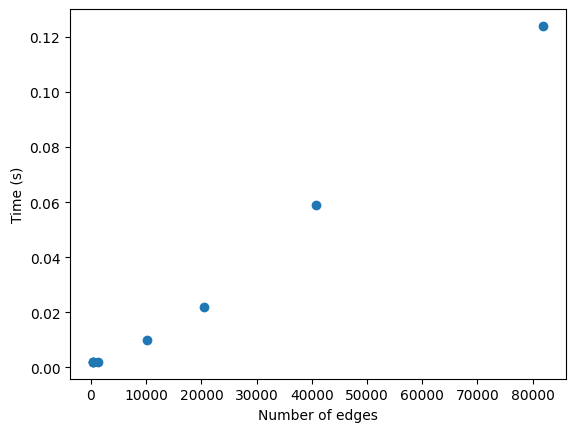
\includegraphics[width=0.6\textwidth]{scat-rand.png}
	\caption{randgen.cのパラメータと実行結果のプロット}
	\label{fig:scatter}
\end{figure}

この図から,グラフの辺の数がある程度多くなると,CPU時間がほぼ線形に増加しているように見える.
これは,増加道を見つけてそれらを反転させる操作を行う回数が,グラフの辺の数が増えていくほど増加するためであると考えられる.

また,辺の数が少ない間はほとんどCPU時間に差が見られないので,グラフの辺の数がある程度小さい間はファイルの中身を読み取ったりグラフを構築したり
する操作にかかる時間の影響が大きいと考えられる.d

% \bibliography{hoge} %hoge.bibから拡張子を外した名前
% \bibliographystyle{junsrt} %参考文献出力スタイル
% 使用する際は latex-workshop.latex.recipe.default を
% ptex2pdf (uplatex) → bibtex → ptex2pdf (uplatex) × 2
% に変更

\end{document}
